\begin{figure}[h]
    \centering
    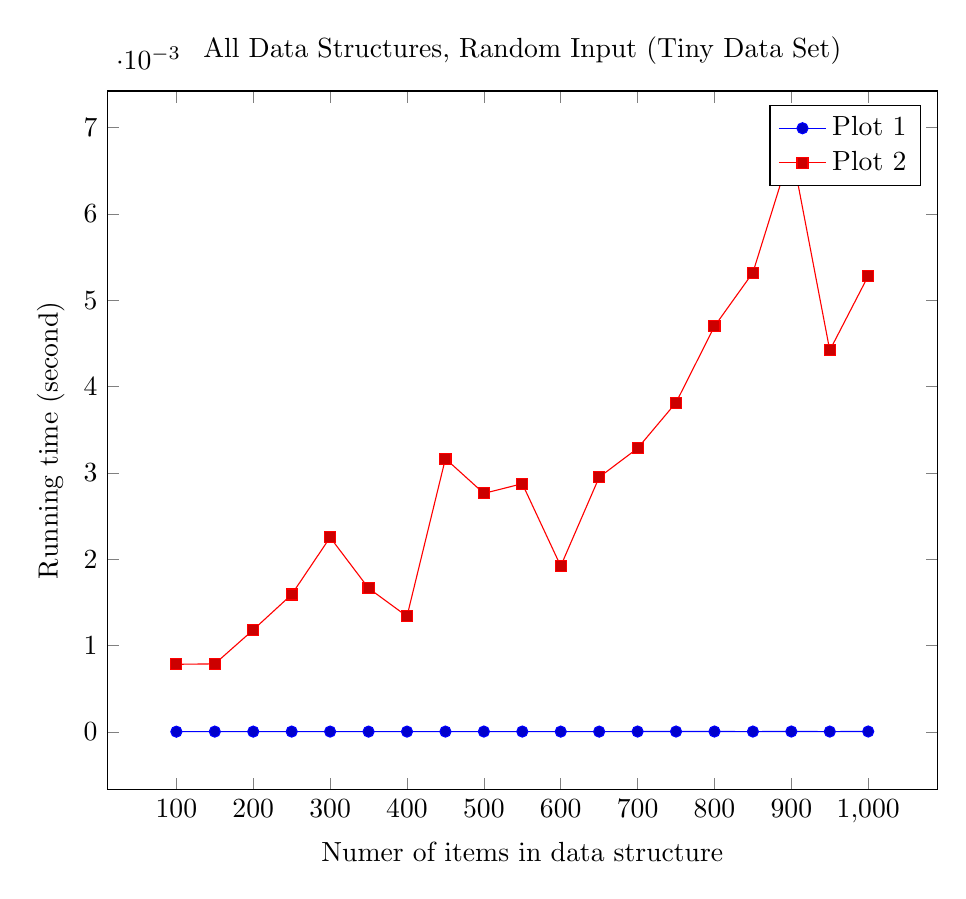
\begin{tikzpicture}
        \begin{axis}[
            xlabel={Numer of items in data structure},
            ylabel={Running time (second)},
            title={All Data Structures, Random Input (Tiny Data Set)},
            width=\textwidth
        ]
		\addplot coordinates {
			(100, 3.4032813052939098e-06)
			(150, 4.156219647173095e-06)
			(200, 4.005631978797254e-06)
			(250, 4.306807315548932e-06)
			(300, 4.367042382899251e-06)
			(350, 3.975514445122099e-06)
			(400, 4.18633718084825e-06)
			(450, 4.306807315548932e-06)
			(500, 4.728452787001276e-06)
			(550, 4.577865118625445e-06)
			(600, 3.945396911446885e-06)
			(650, 3.975514445122078e-06)
			(700, 4.939275522727448e-06)
			(750, 5.0296281237529815e-06)
			(800, 4.9091579890522995e-06)
			(850, 4.607982652300637e-06)
			(900, 5.180215792128726e-06)
			(950, 4.547747584950253e-06)
			(1000, 5.270568393154259e-06)
		};
		\addplot coordinates {
			(100, 0.0007838690489635799)
			(150, 0.0007883565614811808)
			(200, 0.0011826553123564705)
			(250, 0.0015918020073336175)
			(300, 0.0022533938695760204)
			(350, 0.0016648370264959022)
			(400, 0.001338965312130591)
			(450, 0.003165172084058032)
			(500, 0.00276241030622002)
			(550, 0.002874658354227366)
			(600, 0.001920896297802166)
			(650, 0.002949681130612225)
			(700, 0.0032847085752147898)
			(750, 0.0038139037594211445)
			(800, 0.004696889611709709)
			(850, 0.005319057622371304)
			(900, 0.0067481044777243145)
			(950, 0.0044186337180848415)
			(1000, 0.005280326474065023)
		};
        \legend{Plot 1, Plot 2}
        \end{axis}
    \end{tikzpicture}
    \caption{Average of 10 operations, benchmarked every 50, starting at 100.}
\end{figure}